% !TeX root = ../main.tex
\chapter{Project 05: Distributed Target localization under sparse sensor attacks}

\section{Objectives}
The aim of this project is to localize the position of a device using RSS fingerprinting setting. However, unlike the second project, this time the aim is to do the task using distributed consensus-based optimization by nodes. In this project, we are given the dictionary $D$, and it is requested to localize the position of the device having a given measurement which is corrupted by attacks.

\section{Setting of the problem}
The localization problem is set in 10 by 10 squaremeters room. The room is gridded into 100 cells and 20 sensors are used in the training phase. In addition, it is assumed that during the training step has done in an offline manner, and therefore, the dictionary $D$ is assumed to be attack free. The difference in this setting is that each node knows its own row in the matrix $D$ and the matrix $D$ is not known globally, due to privacy matters. It is assumed that the sensors enjoy computational power and therefore they update their own state and share it with their neighbors. Further, a matrix $Q$ is given, determining the topology of the network, or the weights by which the nodes perform the average of theshared states of their neighbors. The communication link are assumed to be secure and only the sensors are under the attack. The number of attacked sensors the same as the project 2 is 5.
\begin{figure}[H] % h means "here", can also use t (top), b (bottom), p (page)
    \centering
    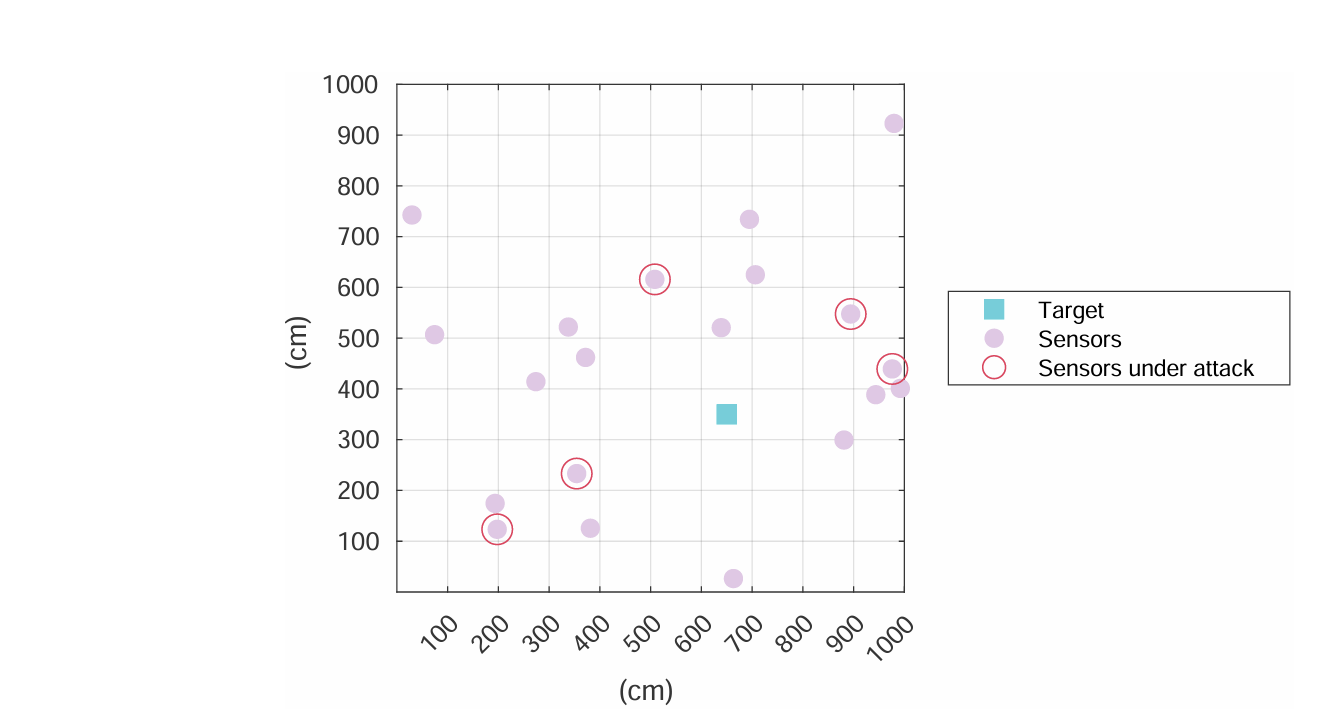
\includegraphics[width=0.75\textwidth]{localization_setting.png} % Adjust width as needed
    \caption{The graphical setting of the problem; reported from the project 2025 file.}
\end{figure}
The dimensions of the problem are as follows:
\begin{itemize}
	\item the number of the cells (states) $n = 100$,  states can be 0 or 1, and only 1 state can be 1.
	\item the number of the sensors, or nodes, length of the measurement sensor $q = 20$, 
	\item the number of the attacks $h = 5$
\end{itemize}

It is required to solve the problem considering two network topology: star and ring. The relaxed problem to be solved in order to solve the distributed consensus-based optimization problem is going to be as follows:

\begin{equation}
\min_{\{x^{(i)}, a^{(i)}\}_{i=1}^q} 
\sum_{i=1}^q \left\| C x^{(i)} + a^{(i)} - y^{(i)} \right\|_2^2
+ \lambda_1 \sum_{i=1}^q \left\| x^{(i)} \right\|_1
+ \lambda_2 \sum_{i=1}^q \left\| a^{(i)} \right\|_1
+ \frac{\lambda}{2} \sum_{i,j \in \mathcal{N}(i)} \left\| x^{(i)} - x^{(j)} \right\|_2^2
\end{equation}


\section{Implementation of the algorithm}
\subsection{DISTA for Ring Topology}
The topology of the network in the ring problem is as follows:
\begin{figure}[H] % h means "here", can also use t (top), b (bottom), p (page)
    \centering
    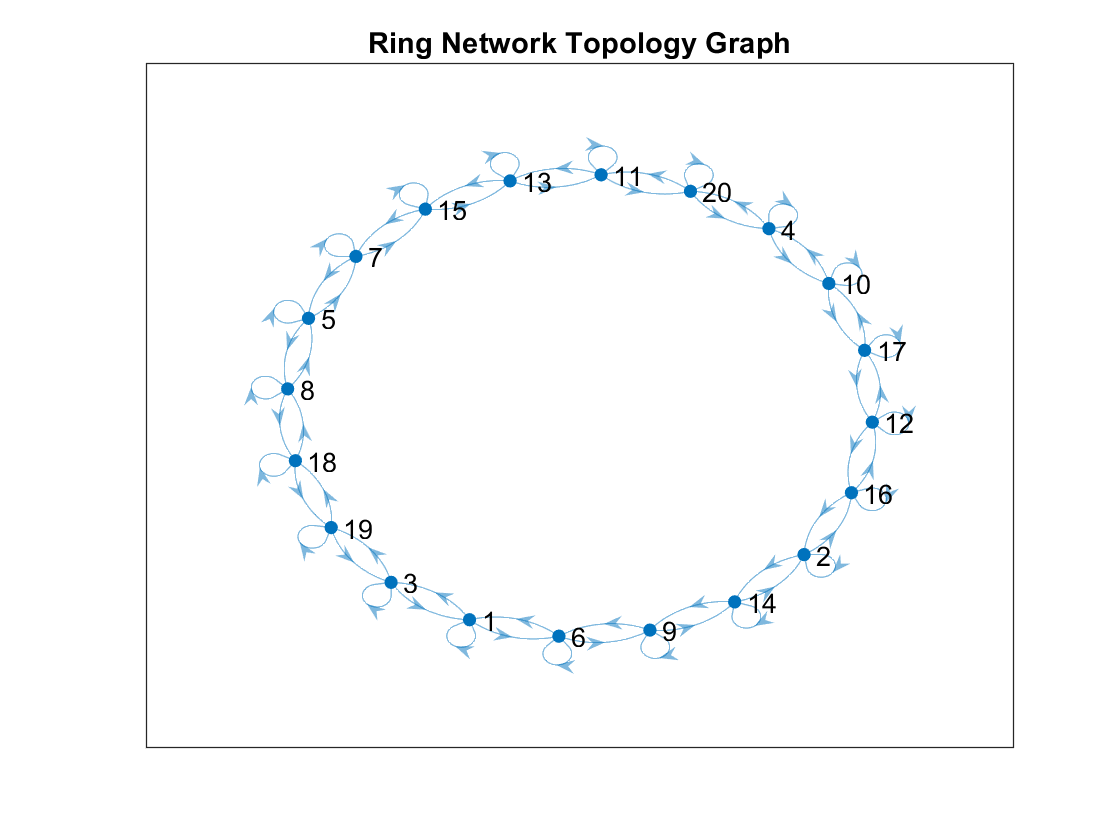
\includegraphics[width=0.75\textwidth]{ring-topology.png} % Adjust width as needed
    \caption{The graph of the communication link in Ring topology.}
\end{figure}
In this topology each node has the same number of data with which they communicate. 

The iterative algorithm to use for solving the problem is DISTA, with the difference that since the state is also sparse, it is needed to apply soft-thresholding to both the states and the attack.

\begin{equation}
\begin{pmatrix}
x^{(i)}(k+1) \\
a^{(i)}(k+1)
\end{pmatrix}
=
\mathcal{S}_{\nu \lambda} \left[
\sum_{j=1}^{q} Q_{i,j}
\begin{pmatrix}
x^{(j)}(k) \\
a^{(j)}(k)
\end{pmatrix}
-
\nu G^{(i)\top} \left( y^{(i)} -
G^{(i)}
\begin{pmatrix}
x^{(i)}(k) \\
a^{(i)}(k)
\end{pmatrix}
\right)
\right]
\end{equation}


The suggested parameters for this problem is:
\begin{itemize}
	\item $\lambda = 1$
	\item $\nu = 0.01*\|G\|_2^{-2}$
\end{itemize}

This algorithm is run until the difference of the two consequitive states becomes lower that $\delta = 10^{-8}$.

Once this goal is achieved, the state position needs to be cleaned. That is, 0 should be allocated to the states with values smaller than a certain threshold, and 1 should be allocated otherwise. Since we know that we have one target to track, we can simply allocate 1 to the maximum of the state for each node. Regarding the attacks, a threshold of 0.05 is used in the Ring topology. It is,further, expected that at the end of the simulation, a consensus is reached in the network, thereby all the nodes have the same estimation of the position of the target, as well as the position of the attacked sensors.

\subsection{DISTA for Star Topology}
The topology of the network in the star problem is as follows:
\begin{figure}[H] % h means "here", can also use t (top), b (bottom), p (page)
    \centering
    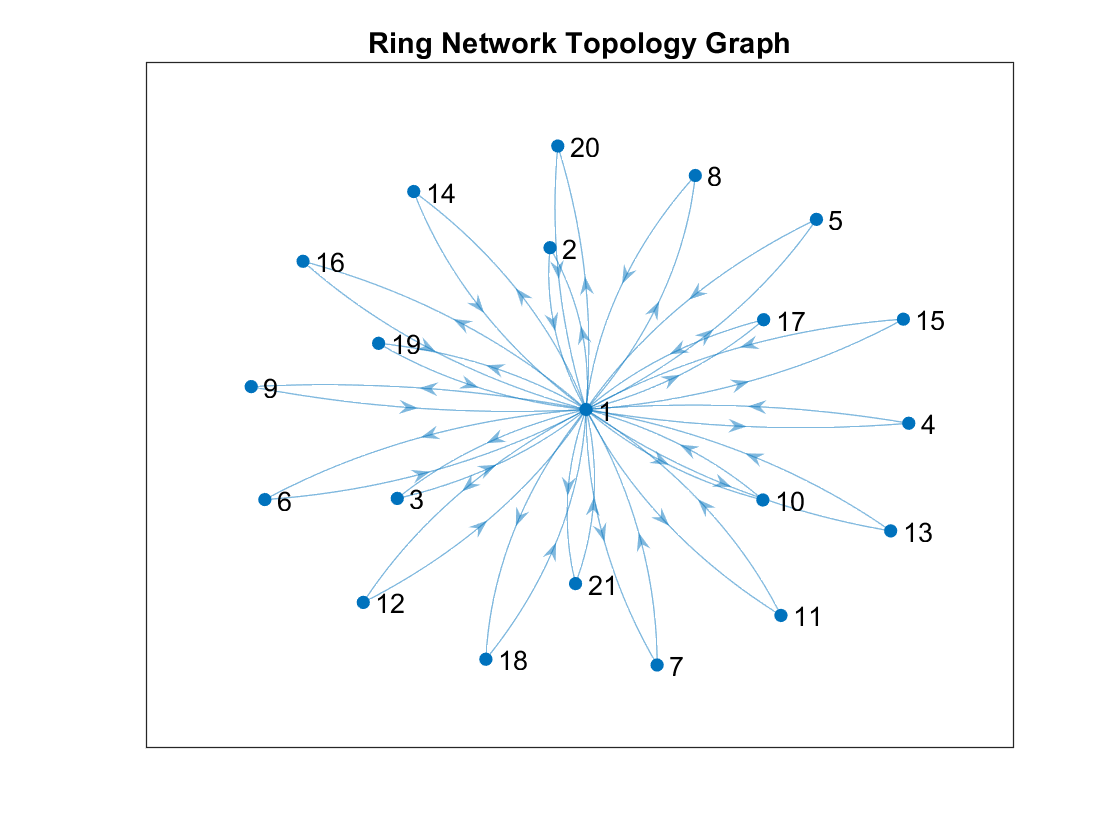
\includegraphics[width=0.75\textwidth]{star-topology.png} % Adjust width as needed
    \caption{The graph of the communication link in Star topology; the node zero at each iteration computes the average state of all the nodes and transmit it to all the nodes to perform their calculations.}
\end{figure}
In this configuration, there is one super node, node 0, where it receives the state of all the nodes, calculate the mean, and send the calculated average of the states to the nodes. Afterwards, each node perform distributed gradient descent modifying the average state received from the super node.

The same algorithm of the Ring topology is used here. However, before updating the states, the mean is calculated by the super node, and then the nodes perform the calculations.
\begin{equation}
\begin{pmatrix}
x^{0}(k) \\
a^{0}(k)
\end{pmatrix} = \sum_{j=1}^{q} Q_{1,j}^{j} \begin{pmatrix}
x^{j}(k) \\
a^{j}(k)
\end{pmatrix}
\end{equation}

\begin{equation}
\begin{pmatrix}
x^{(i)}(k+1) \\
a^{(i)}(k+1)
\end{pmatrix}
=
\mathcal{S}_{\nu \lambda} \left(
\sum_{j=1}^{q} Q_{i,j}
\begin{pmatrix}
x^{(j)}(k) \\
a^{(j)}(k)
\end{pmatrix}
-
\nu G^{(i)\top} \left( y^{(i)} -
G^{(i)}
\begin{pmatrix}
x^{(i)}(k) \\
a^{(i)}(k)
\end{pmatrix}
\right)
\right)
\end{equation}

The suggested parameters for this problem is:
\begin{itemize}
	\item $\lambda = 1$
	\item $\nu = 0.01*\|G\|_2^{-2}$
\end{itemize}

This algorithm is run until the difference of the two consequitive states becomes lower that $\delta = 10^{-8}$.

The same as the Ring topology, after the algorithm stops, we need to clean the data. The cleaning threshold for the attack is 0.07 for the star topology.

In an attemp to enhance the performance of the algorithm the following values were used as hyperparameters:
\begin{itemize}
	\item $\nu = 0.012*\|G\|_2^{-2}$
	\item $\lambda= 1.3$
\end{itemize}


\section{Results}
It was observed that both Ring and Star topology reached the consensus after a finite number of iterations. Furthermore, all the nodes correctly estimated the position of the target and the attacked nodes. In the following plots suggesting this result is represented. 
\begin{figure}[H]
    \centering
    \subfloat[The head map of the state support vector of different nodes after the consensus in the Ring topology.]{
        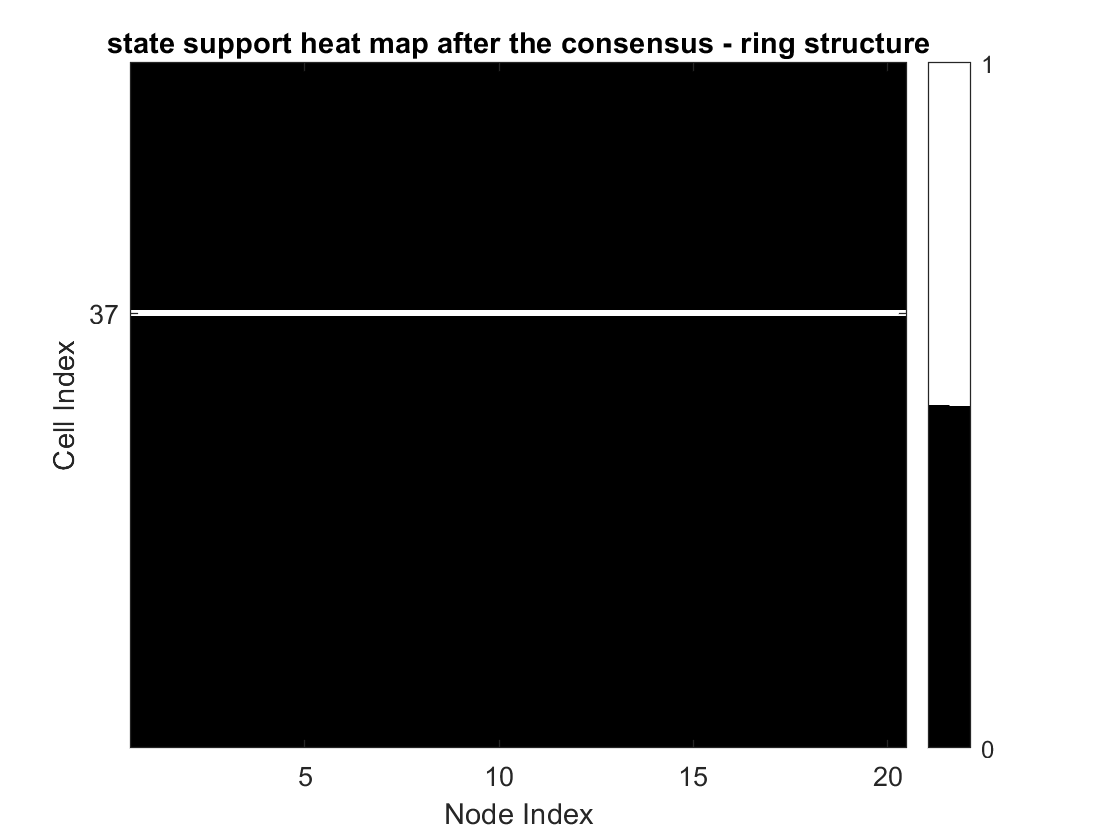
\includegraphics[width=0.45\textwidth]{state-ring.png} % Adjust width as needed
    }
    \hspace{1cm} % Adjust the space between the two figures
    \subfloat[The head map of the attack support vector of different nodes after the consensus in the Ring topology.]{
        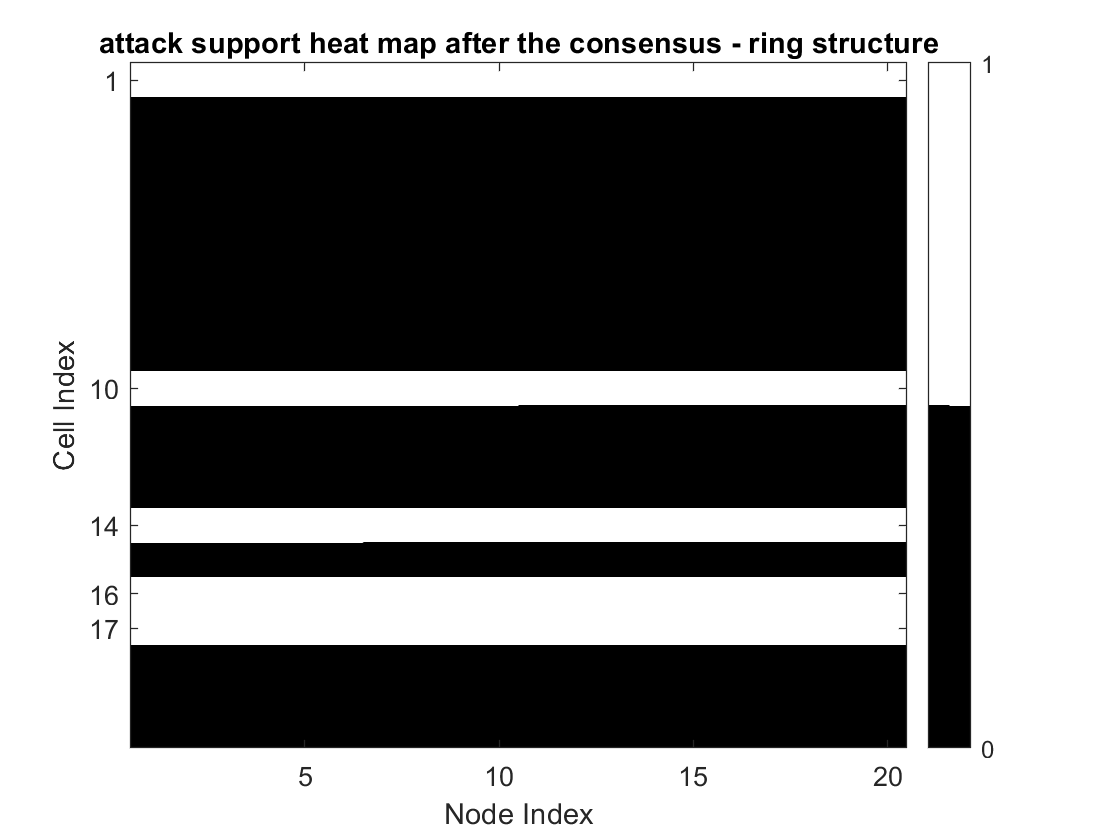
\includegraphics[width=0.45\textwidth]{attack-ring.png} % Adjust width as needed
    }
    \caption{Comparison of state and attack support vectors after consensus in the Ring topology.}
\end{figure}

\begin{figure}[H]
    \centering
    \subfloat[The head map of the state support vector of different nodes after the consensus in the Star topology.]{
        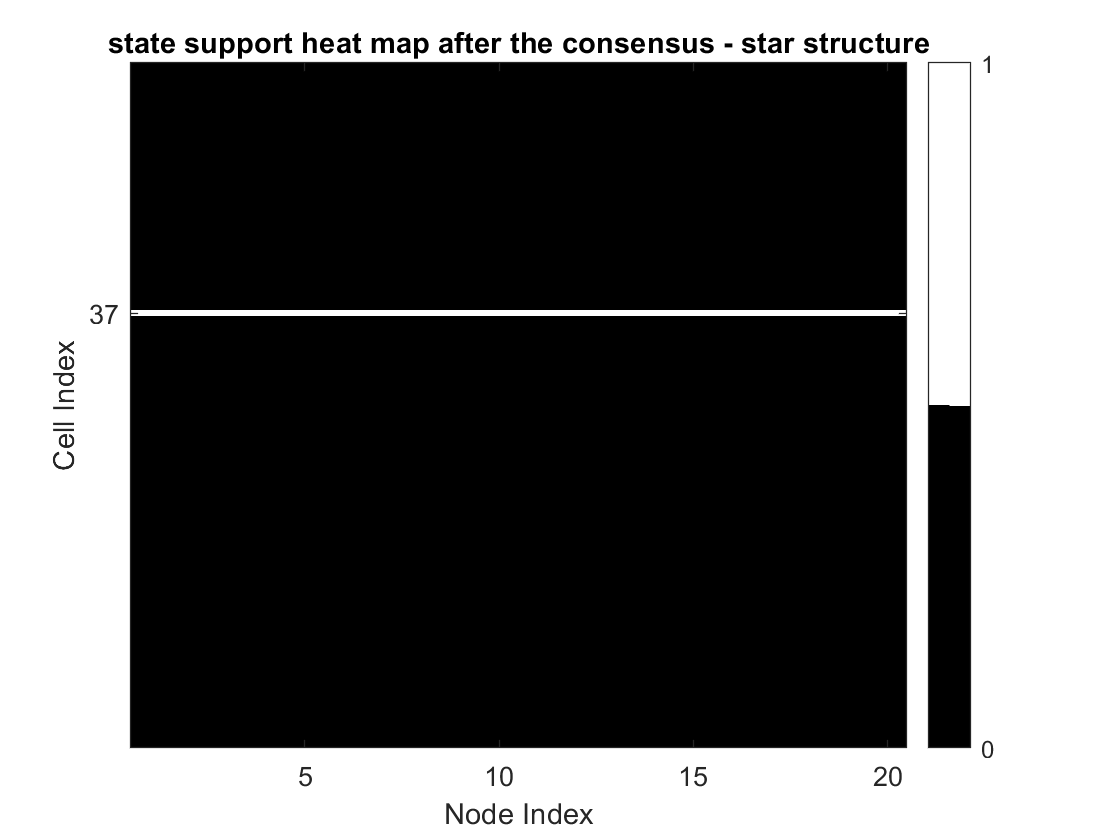
\includegraphics[width=0.45\textwidth]{state-star.png} % Adjust width as needed
    }
    \hspace{1cm} % Adjust the space between the two figures
    \subfloat[The head map of the attack support vector of different nodes after the consensus in the Star topology.]{
        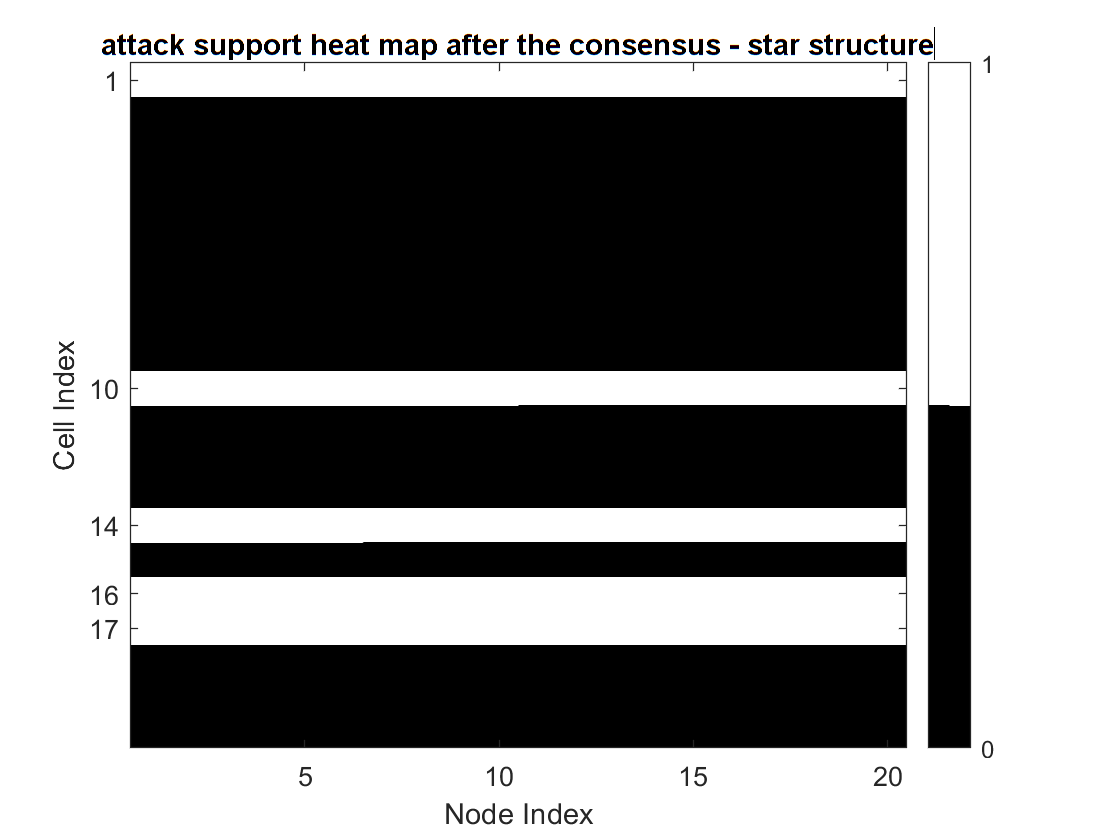
\includegraphics[width=0.45\textwidth]{attack-star.png} % Adjust width as needed
    }
    \caption{Comparison of state and attack support vectors after consensus in the Star topology.}
\end{figure}

In terms of the number of iteration to reahing consensus, both topologies reach consensus in the same order of magnitude; however, ring topology reaches consensus a bit faster. The number of iterations to reach consensus with suggested and enhance parameters can be seen in the following figure.
\begin{figure}[H] % h means "here", can also use t (top), b (bottom), p (page)
    \centering
    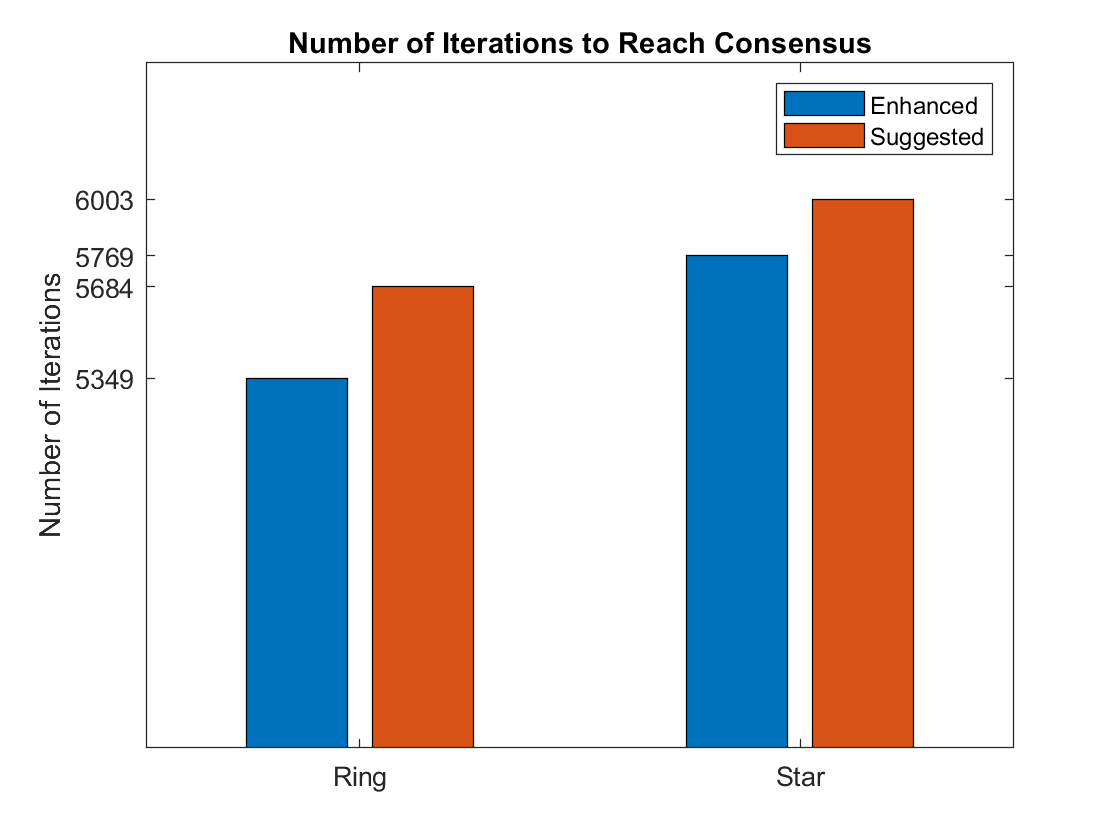
\includegraphics[width=0.45\textwidth]{iteration.png} % Adjust width as needed
    \caption{The number of iterations to reach consensus.}
\end{figure}

A distributed IJAM algorithm may not work well for states with sparse values, due to the fact that this algorithm does enjoy a smooth transient for state estimation, and when a soft-thresholding is applied to the term including the state, the network may not reach a consensus or it may take a large amount of iterations to reach so.

\section{Further discussion}
Consdering the tracking problem the estimation can be enhanced in the following way: after a node realized that its sensor is under attack, it can cutoff the term updating its update based on its measurement, and continue with making the average of the other states, until the sensor reaches a consensus. Therefore, after the attacked nodes stop taking into considerations their measurement, the problem changes to the following format:

\begin{equation}
\min_{x^{(1)}, \dots, x^{(q)}} 
\sum_{i=1,\:\: i\neq\text{attacked sensors}}^q \left\| C x^{(i)} + a^{(i)} - y^{(i)} \right\|_2^2
+ \lambda_1 \sum_{i=1}^q \left\| x^{(i)} \right\|_1
+ \lambda_2 \sum_{i=1}^q \left\| a^{(i)} \right\|_1
+ \frac{\lambda}{2} \sum_{i,j \in \mathcal{N}(i)} \left\| x^{(i)} - x^{(j)} \right\|_2^2
\end{equation}


Since the node keeps on performing averaging, the consensus in the network is going to be guaranteed. Further, since the only measurements that remain are attack-free measurement, the estimation is expected to be more accurate.


\section{Conclusion}
DISTA is capable of providing consensus to the network in both Star and Ring topology. Therefore, all the nodes located the position of the target correctly after the consensus. In addition, they were able to detect the position of the attacked nodes accurately. Ring topology has the advantage that it reaches consensus in smaller number of iteration. 

The reason that IJAM is not used in this process is that it does not enjoy a smooth transient and when soft-thresholding is applied to it, which is the case for this project, the algorithm either the network does not reach a consensu or it reaches in a considerably larger number of iterations.

To enhance the estimation in the tracking problem, once a node detects that its sensor is under attack, it can stop updating based on its own measurement and instead rely on averaging the states of other nodes until consensus is reached. This modifies the optimization problem as follows:

\[
\min_{x^{(1)}, \dots, x^{(q)}} 
\sum_{i=1,\:\: i\neq\text{attacked sensors}}^q \left\| C x^{(i)} + a^{(i)} - y^{(i)} \right\|_2^2
+ \lambda_1 \sum_{i=1}^q \left\| x^{(i)} \right\|_1
+ \lambda_2 \sum_{i=1}^q \left\| a^{(i)} \right\|_1
+ \frac{\lambda}{2} \sum_{i,j \in \mathcal{N}(i)} \left\| x^{(i)} - x^{(j)} \right\|_2^2
\]

By continuously averaging, the network can guarantee consensus. Additionally, since only non-attacked measurements are used, the estimation becomes more accurate.









